%% Beginning of file 'PASPsample701.tex'
%%
%% Modified 2025 July  
%%
%% The following template is adapted from the AASTeX "sample701.tex"
%% AAS Journals template.
%%
%% Version 7.0.1. Created May 2025.
%% Version 7. Created January 2025.  
%%
%% AASTeX v7+ calls the following external packages:
%% times, hyperref, ifthen, hyphens, longtable, xcolor, 
%% bookmarks, array, rotating, ulem, and lineno 
%%
%% RevTeX is no longer used in AASTeX v7+.
%%
\documentclass[linenumbers,trackchanges]{aastex701}
%%
%% This initial command takes arguments that can be used to easily modify 
%% the output of the compiled manuscript. Any combination of arguments can be 
%% invoked like this:
%%
%% \documentclass[argument1,argument2,argument3,...]{aastex7}
%%
%% Six of the arguments are typestting options. They are:
%%
%%  twocolumn   : two text columns, 10 point font, single spaced article.
%%                This is the most compact and represent the final published
%%                derived PDF copy of the accepted manuscript from the publisher
%%  default     : one text column, 10 point font, single spaced (default).
%%  manuscript  : one text column, 12 point font, double spaced article.
%%  preprint    : one text column, 12 point font, single spaced article.  
%%  preprint2   : two text columns, 12 point font, single spaced article.
%%  modern      : a stylish, single text column, 12 point font, article with
%% 		  wider left and right margins. This uses the Daniel
%% 		  Foreman-Mackey and David Hogg design.
%%
%% Note that you can submit to PASP in any of these 6 styles.
%%
%% There are other optional arguments one can invoke to allow other stylistic
%% actions. The available options are:
%%
%%   astrosymb    : Loads Astrosymb font and define \astrocommands. 
%%   tighten      : Makes baselineskip slightly smaller, only works with 
%%                  the twocolumn substyle.
%%   times        : uses times font instead of the default.
%%   linenumbers  : turn on linenumbering. Note this is mandatory for PASP
%%                  submissions and revisions.
%%   trackchanges : Shows added text in bold.
%%   longauthor   : Do not use the more compressed footnote style (default) for 
%%                  the author/collaboration/affiliations. Instead print all
%%                  affiliation information after each name. Creates a much 
%%                  longer author list but may be desirable for short 
%%                  author papers.
%% twocolappendix : make 2 column appendix.
%%   anonymous    : Do not show the authors, affiliations, acknowledgments,
%%                  and author contributions for dual anonymous review.
%%  resetfootnote : Reset footnotes to 1 in the body of the manuscript.
%%                  Useful when there are a lot of authors and affiliations
%%		    in the front matter.
%%   longbib      : Print article titles in the references. This option
%% 		    is mandatory for PSJ manuscripts.
%%
%% Since v6, AASTeX has included \hyperref support. While we have built in 
%% specific %% defaults into the classfile you can manually override them 
%% with the \hypersetup command. For example,
%%
%% \hypersetup{linkcolor=red,citecolor=green,filecolor=cyan,urlcolor=magenta}
%%
%% will change the color of the internal links to red, the links to the
%% bibliography to green, the file links to cyan, and the external links to
%% magenta. Additional information on \hyperref options can be found here:
%% https://www.tug.org/applications/hyperref/manual.html#x1-40003
%%
%% The "bookmarks" has been changed to "true" in hyperref
%% to improve the accessibility of the compiled pdf file.
%%
%% If you want to create your own macros, you can do so
%% using \newcommand. Your macros should appear before
%% the \begin{document} command.
%%
\newcommand{\vdag}{(v)^\dagger}
\newcommand\aastex{AAS\TeX}
\newcommand\latex{La\TeX}

\usepackage{graphicx}
%%%%%%%%%%%%%%%%%%%%%%%%%%%%%%%%%%%%%%%%%%%%%%%%%%%%%%%%%%%%%%%%%%%%%%%%%%%%%%%%
%%
%% The following section outlines numerous optional output that
%% can be displayed in the front matter or as running meta-data.
%%
%% Running header information. A short title on odd pages and 
%% short author list on even pages. Note that this
%% information may be modified in production.
%%\shorttitle{AASTeX v7.0.1 Sample article}
%%\shortauthors{The Terra Mater collaboration}
%%
%% Include dates for submitted, revised, and accepted.
%%\received{February 1, 2025}
%%\revised{March 1, 2025}
%%\accepted{\today}
%%
%% Indicate that article was submitted to PASP.
%%\submitjournal{PASP}
%% Note that this command adds "Submitted to " the argument.
%%
%% You can add a light gray and diagonal water-mark to the first page 
%% with this command:
%% \watermark{text}
%% where "text", e.g. DRAFT, is the text to appear.  If the text is 
%% long you can control the water-mark size with:
%% \setwatermarkfontsize{dimension}
%% where dimension is any recognized LaTeX dimension, e.g. pt, in, etc.
%%%%%%%%%%%%%%%%%%%%%%%%%%%%%%%%%%%%%%%%%%%%%%%%%%%%%%%%%%%%%%%%%%%%%%%%%%%%%%%%
%%
%% Use this command to indicate a subdirectory where figures are located.
%%\graphicspath{{./}{figures/}}
%% This is the end of the preamble.  Indicate the beginning of the
%% manuscript itself with \begin{document}.

\begin{document}

\title{A machine learning approach to detecting anomalities in MWA observations}

%% A significant change from AASTeX v6+ is in the author blocks. Now an email
%% address is required for each author. This means that each author requires
%% at least one of the following:
%%
%% \author
%% \affiliation
%% \email
%%
%% If these three commands are not available for each author, the latex
%% compiler will issue an error and if you force the latex compiler to continue,
%% it will generate an incomplete pdf.
%%
%% Multiple \affiliation commands are allowed and authors can also include
%% an optional \altaffiliation to indicate a status, i.e. Hubble Fellow. 
%% while affiliations are indexed as footnotes, altaffiliations are noted with
%% with a non-numeric footnote that is set away from the numeric \affiliation 
%% footnotes. NOTE that if an \altaffiliation command is used it must 
%% come BEFORE the \affiliation call, right after the \author command, in 
%% order to place the footnotes in the proper location. Because non-numeric
%% symbols are used, \altaffiliation should be used sparingly.
%%
%% In v7+ the \author command takes an optional argument which provides 
%% additional metadata about the author. Authors can provide the 16 digit 
%% ORCID, the surname (family or last) name, the given (first or fore-) name, 
%% and a name suffix, e.g. "Jr.". The syntax is:
%%
%% \author[orcid=0000-0002-9072-1121,gname=Gregory,sname=Schwarz]{Greg Schwarz}
%%
%% This name metadata in not shown, it is only for parsing by the peer review
%% system so authors can be more easily identified. This name information will
%% also be sent to the publisher so they can include it in the CROSSREF 
%% metadata. Including an orcid will hyperlink the author name to the 
%% author's ORCID page. Note that  during compilation, LaTeX will do some 
%% limited checking of the format of the ID to make sure it is valid. If 
%% the "orcid-ID.png" image file is  present or in the LaTeX pathway, the 
%% ORCID icon will appear next to the authors name.
%%
%% Even though emails are now required for each author, the \email does not
%% produce output in the compiled manuscript unless the optional "show" command
%% is used. For example,
%%
%% \email[show]{greg.schwarz@aas.org}
%%
%% All "shown" emails are show in the bottom left of the first page. Due to
%% space constraints, only a few emails should be shown. 
%%
%% To identify a corresponding author, use the \correspondingauthor command.
%% The command appends "Corresponding Author: " to the argument it appears at
%% the bottom left of the first page like the output from \email. 

\author[0000-0003-1183-9293]{Ridhima Nunhokee}
%\altaffiliation{PASP Editor-in-Chief}
\affiliation{Curtin Institute of Radio Astronomy, 1 Turner Avenue, Bentley WA 6102}
\email{cnunhokee@gmail.com}


%% Use the \collaboration command to identify collaborations. This command
%% takes an optional argument that is either a number or the word "all"
%% which tells the compiler how many of the authors above the command to
%% show. For example "\collaboration[all]{(DELVE Collaboration)}" wil include
%% all the authors above this command.
%%
%% Mark off the abstract in the ``abstract'' environment. 
\begin{abstract}

Detecting the cosmological 21 cm signal from the Epoch of Reionization (EoR) remains one of the most challenging objectives in modern radio astronomy. The signal is extremely faint and highly susceptible to contamination arising from instrumental artefacts, calibration failures, radio frequency interference, and other observational systematics. Undetected anomalies within observational datasets can bias downstream scientific analysis and potentially lead to false astrophysical interpretations.

This study investigates the use of machine learning approaches for identifying systematically contaminated observations using calibration-derived metrics obtained during radio telescope processing pipelines. Both unsupervised anomaly detection and supervised classification techniques were evaluated using a dataset containing 12,298 observations characterized by calibration quality metrics. Initial experiments using Isolation Forest demonstrated limited sensitivity in detecting subtle anomalies due to class imbalance and overlapping feature distributions. Supervised approaches including XGBoost, LightGBM, logistic regression, and random forest achieved substantially improved detection performance.

To improve sensitivity toward hidden systematics not captured by existing labels, a hybrid anomaly detection framework combining Isolation Forest, Local Outlier Factor, and Principal Component Analysis reconstruction error is proposed. Results demonstrate that calibration metrics contain meaningful information for identifying systematically contaminated observations and highlight the importance of automated anomaly detection frameworks for improving the reliability of future EoR observations.

\end{abstract}

%% Keywords should appear after the \end{abstract} command. 
%% PASP uses Unified Astronomy Thesaurus (UAT) concepts:
%% https://astrothesaurus.org
%% You will be asked to selected these concepts during the submission process
%% but this old "keyword" functionality is maintained in case authors want
%% to include these concepts in their preprints.
%%
%% You can use the \uat command to link your UAT concepts back its source.
%\keywords{\uat{Galaxies}{573} --- \uat{Cosmology}{343} --- \uat{High Energy astrophysics}{739} --- \uat{Interstellar medium}{847} --- \uat{Stellar astronomy}{1583} --- \uat{Solar physics}{1476}}

%\keywords{\uat{Classical Novae}{251} --- \uat{Ultraviolet astronomy}{1736} --- \uat{History of astronomy}{1868} --- \uat{Interdisciplinary astronomy}{804}}

%% From the front matter, we move on to the body of the paper.
%% Sections are demarcated by \section and \subsection, respectively.
%% Observe the use of the LaTeX \label
%% command after the \subsection to give a symbolic KEY to the
%% subsection for cross-referencing in a \ref command.
%% You can use LaTeX's \ref and \label commands to keep track of
%% cross-references to sections, equations, tables, and figures.
%% That way, if you change the order of any elements, LaTeX will
%% automatically renumber them.

\section{Introduction} \label{sec:Intro}
One of the primary goals of contemporary radio astronomy is the detection of the redshifted 21 cm hydrogen signal originating from the Epoch of Reionization, a period marking the formation of the first luminous structures in the early universe. Experiments associated with instruments such as the Square Kilometre Array Observatory (SKA), Murchison Widefield Array (MWA), and other low-frequency interferometers aim to measure this signal.

However, the EoR signal is several orders of magnitude weaker than astrophysical foregrounds and highly vulnerable to contamination introduced by systematic effects. Calibration errors, unstable instrumental gain solutions, receiver noise variation, and incomplete convergence during signal processing can introduce biases that propagate into later stages of analysis.

Traditional quality control procedures often rely on manual inspection or predefined threshold-based filtering. These approaches become increasingly inefficient as observational datasets continue to grow in scale. Machine learning provides a potential solution by enabling automated identification of anomalous observations that may contain hidden systematic contamination.

This work explores the use of machine learning models to detect systematically dominated observations using calibration-derived quality metrics extracted from radio astronomy processing pipelines.

\section{Motivation} \label{sec:motivation}

Unlike conventional radio astronomy imaging, EoR experiments rely on statistical detection of an extremely weak signal buried beneath bright foreground emission. The scientific challenge is not simply removing foregrounds, but ensuring that instrumental systematics do not create artificial spectral signatures that become indistinguishable from the cosmological signal.

Calibration anomalies can affect EoR science in several ways:

Spectral contamination from gain errors introduces frequency-dependent artifacts that leak into high-delay Fourier modes.
Incomplete calibration convergence results in incorrect antenna gain solutions that propagate systematic errors into visibilities.
Receiver instabilities introduce time-dependent fluctuations that bias power spectrum estimation.
Baseline corruption affects uv-coverage consistency and distorts image reconstruction.
Residual systematic structures can mimic large-scale 21 cm fluctuations, producing false positive detections.

Since EoR power spectrum estimation assumes extremely well-characterized instrument behaviour, even a small number of poor-quality observations can bias final cosmological measurements.

Traditional quality control methods often rely on manual inspection or hard-threshold rejection criteria. However, modern telescopes generate observational datasets at scales where manual analysis becomes impractical. Automated anomaly detection therefore becomes essential.

\section{Dataset and Calibration Metrics}

This study used 12,298 observations obtained during calibration processing stages. Several calibration diagnostics were extracted as machine learning features representing instrumental and calibration stability.

The selected features include:
\begin{itemize}
\item $RMS\,CONVG$: Root mean square convergence metric measuring calibration stability.
\item $SKEW$: Statistical skewness of calibration solutions, indicating asymmetry or instability in gain distributions.
\item $RECV\,VAR$: Receiver variance across antennas and frequency channels representing instrumental noise fluctuations.
\item $DFFT\,POW$: Delay-domain Fourier transform power sensitive to spectral structure contamination.
\item $BL\,UNUSED\,FRAC$: Fraction of interferometric baselines rejected during calibration.
\item $NON\,CONVG\,CHS\,FRAC$: Fraction of frequency channels where calibration solutions failed to converge.
\end{itemize}
These metrics provide a quantitative description of calibration quality and potential systematic contamination. The dataset is inherently imbalanced, consisting of:
\begin{itemize}
\item Good observations: 11,108 (90.3\%)
\item Failed observations: 1,190 (9.7\%)
\end{itemize}
This class imbalance presents a significant challenge for anomaly detection.

\section{Unsupervised Anomaly Detection Using Isolation Forest}
The first stage of this study employed the Isolation Forest algorithm, an unsupervised anomaly detection technique specifically designed to identify rare and abnormal observations without requiring labeled training data. Unlike conventional classification algorithms, Isolation Forest operates on the principle that anomalous observations are ``few and different''. Rather than learning a decision boundary between classes, the algorithm isolates observations by recursively partitioning the feature space using randomly selected features and split values.

The algorithm constructs an ensemble of binary decision trees, referred to as isolation trees. During tree construction, each split randomly selects:
\begin{itemize}
\item A feature from the available feature set
\item A random split value within the range of that feature
\end{itemize}
An observation is considered anomalous if it can be isolated after a relatively small number of splits. In contrast, normal observations located within dense clusters require a greater number of partitioning steps. The anomaly score is determined from the average path length across all isolation trees. Mathematically, the anomaly score is defined as
\begin{equation}
s(x,n)=2^{-\frac{E(h(x))}{c(n)}}
\end{equation}
where$h(x)$ is the path length required to isolate observation $x$, $E(h(x))$ is the average path length over all trees and $c(n)$ is the average path length normalization factor for a dataset of size $n$. Observations with shorter path lengths produce anomaly scores closer to 1 and are therefore classified as anomalous.

Isolation Forest was selected because calibration failures in radio astronomy often manifest as unusual combinations of calibration metrics that deviate from the expected statistical behavior of normal observations. The algorithm is computationally efficient and suitable for large-scale observational datasets where labeled anomaly examples may be limited.

Initial contamination estimation was set at 5.5\%. Performance evaluation yielded the confusion matrix illustrated in Table~\ref{tab:table1}. The resulting performance metrics were: Precision of 46\%, Recall	of 26\% and F1-Score of 33\%.

\begin{table}
\label{tab:table1}
\centering
\caption{Isolation Forest Confusion Matrix}
\begin{tabular}{ccc}
 & Predicted Normal & Predicted Anomaly \\
 \toprule \\
Actual Normal & 10384 & 878 \\
Actual Anomaly & 684 & 366 \\
\end{tabular}
\end{table}

Several limitations were observed during unsupervised anomaly detection.
First, the dataset exhibits severe class imbalance, causing anomalous observations to remain underrepresented during tree construction. Second, many systematic failures appear to be subtle rather than extreme outliers, reducing the effectiveness of purely distance-based anomaly detection.

Increasing contamination estimation to the true anomaly rate of 9.7\% improved recall to 42\%, but introduced additional false positives. Application of robust scaling produced minimal improvement. These results suggest that calibration failures are not always represented as obvious outliers in feature space.

\subsection{Supervised Classification}

Although unsupervised anomaly detection can identify unusual observations, many systematic failures in radio astronomy calibration pipelines are subtle and may not appear as extreme statistical outliers. To improve detection performance, supervised classification algorithms were trained using labeled observations categorized as PASS (scientifically acceptable) and FAIL (contaminated observations).

The objective of supervised learning is to learn the relationship between calibration metrics and known observational quality outcomes, allowing the model to predict whether previously unseen observations are likely to contain systematic contamination. The dataset was partitioned using an 80:20 training-testing split. Several classification algorithms were evaluated:
\begin{enumerate}
\item Random Forest
\item Logistic Regression
\item XGBoost
\item LightGBM
\item Isolation Forest (baseline comparison)
\end{enumerate}
Performance results are summarized in Table~\ref{tab:table2}.
\begin{table}
\label{tab:table2}
\centering
\caption{Isolation Forest Performance Metrics}
\begin{tabular}{ccccc}
Random Forest	& 1.00 &	1.00	 & 1.00\\
Logistic Regression	& 0.00	& 0.00 &	0.00\\
XGBoost	& 1.00 &	0.96	& 0.98 \\
LightGBM	& 1.00	& 1.00	& 1.00 \\
Isolation Forest	& 0.03	& 0.43	& 0.05
\end{tabular}
\end{table}

\subsection{Random Forest}
Random Forest is an ensemble learning algorithm that constructs multiple decision trees during training and combines their predictions through majority voting. Each decision tree is trained using a bootstrap sample of the original dataset, while feature selection at each split is randomized. This process reduces overfitting and improves model generalization. For classification, the final prediction is obtained by
\begin{equation}
\hat{y} = mode(T_1(x), T_2(x), ..., T_n(x))
\end{equation}
where $T_i(x)$ represents the prediction from the $i^{th}$ decision tree.

Random Forest is particularly suitable for this problem because it can capture complex nonlinear relationships between calibration metrics while remaining relatively robust to noisy data and feature interactions. Tree-based ensemble methods significantly outperformed unsupervised detection approaches. However, the near-perfect classification performance raises the possibility of data leakage, feature redundancy, or overly correlated labels and requires further validation.

\subsection{Logistic Regression}
Logistic Regression is a probabilistic linear classification algorithm used to estimate the likelihood of an observation belonging to a given class. Unlike tree-based methods, Logistic Regression assumes a linear relationship between input features and the log-odds of class membership. The probability of class membership is modeled using the sigmoid function
\begin{equation}
P(y=1|x)=\frac{1}{1+e^{-(\beta_0+\beta_1x_1+\beta_2x_2+...+\beta_nx_n)}}
\end{equation}
where $\beta_i$ are learned coefficients corresponding to each feature. 

This model serves as a baseline classifier to evaluate whether systematic contamination can be linearly separated using calibration metrics. The poor performance observed suggests that relationships between calibration metrics and failure states are highly nonlinear.

\subsection{XGBoost}
Extreme Gradient Boosting (XGBoost) is an advanced ensemble learning algorithm based on gradient boosting decision trees. Unlike Random Forest, where trees are constructed independently, XGBoost builds trees sequentially. Each new tree attempts to correct errors made by previous trees by minimizing a differentiable loss function.

At each iteration, the model updates according to
\begin{equation}
F_m(x)=F_{m-1}(x)+\eta h_m(x)
\end{equation}
where $F_m(x)$ is the updated model, $h_m(x)$ is the newly trained decision tree and $\eta$ is the learning rate controlling update magnitude.

The optimization objective includes both prediction loss and regularization
\begin{equation}
L=\sum l(y_i,\hat{y_i})+\sum \Omega(f_k)
\end{equation}
where $\Omega$ penalizes model complexity.

XGBoost is particularly effective for identifying systematic contamination because it captures complex nonlinear relationships while handling noisy, heterogeneous, and imbalanced datasets effectively.

\subsection{LightGBM}
Light Gradient Boosting Machine (LightGBM) is a high-performance gradient boosting framework optimized for computational efficiency. Similar to XGBoost, LightGBM builds decision trees sequentially to minimize prediction error. However, it differs in two important ways. First, LightGBM uses histogram-based feature binning to reduce memory usage and computational cost.

Second, instead of growing trees level-wise, LightGBM grows trees leaf-wise, selecting the leaf that maximally reduces loss. The algorithm optimizes an objective function of the form
\begin{equation}
L=\sum l(y_i,\hat{y_i})+\lambda \Omega(T)
\end{equation}
where $\Omega(T)$ represents tree complexity regularization.

LightGBM is particularly useful for large astronomical datasets because radio telescope observations can generate millions of samples, requiring efficient model training while maintaining predictive accuracy.

\section{Hybrid Systematics Detection Framework}
Although supervised learning performs well on known failure patterns, future observations may contain previously unseen systematic contamination. To address this limitation, a hybrid anomaly detection framework was designed using only trusted observations where PASS = True. The framework models normal system behaviour and identifies deviations from learned patterns. Three complementary anomaly detectors were combined: Isolation Forest, Local Outlier Factor (LOF) and Principal Component Analysis Reconstruction Error.

\subsection{Isolation Forest Anomaly Scoring}
Isolation Forest constructs an ensemble of randomly generated binary trees that recursively partition the feature space. The key idea is that anomalies are \emph{easier to isolate} than normal observations. For a given observation $x$, the algorithm computes the path length $h(x)$, defined as the number of splits required to isolate the point within a tree. The expected path length over an ensemble of trees is given by:
\begin{equation}
E[h(x)] = \frac{1}{T} \sum_{t=1}^{T} h_t(x),
\end{equation}
where $T$ is the number of trees. The anomaly score is then defined as:
\begin{equation}
S_{\text{IF}}(x) = 2^{-\frac{E[h(x)]}{c(n)}},
\end{equation}
where $c(n)$ is a normalization constant representing the average path length of unsuccessful searches in a binary search tree:
\begin{equation}
c(n) = 2H(n - 1) - \frac{2(n - 1)}{n},
\end{equation}
and $H(i)$ is the $i$-th harmonic number. Values of $S_{\text{IF}}(x)$ close to 1 indicate strong anomalies, while values near 0.5 correspond to typical observations within dense regions of the data distribution.

The trained anomaly detection framework was applied to the full observational dataset. For each observation, the following anomaly scores were computed:
\begin{itemize}
\item Isolation Forest anomaly score
\item LOF score
\item PCA reconstruction error
\end{itemize}

\subsection{Local Outlier Factor (LOF)}
Local Outlier Factor is a density-based anomaly detection algorithm that identifies observations whose local neighborhood density differs significantly from surrounding observations. Unlike Isolation Forest, which identifies global anomalies, LOF focuses on local inconsistencies. For a given observation, the local density is estimated based on distances to its nearest neighbors. The anomaly score is computed as
\begin{equation}
LOF(x)=\frac{\sum_{o\in N(x)}\frac{lrd(o)}{lrd(x)}}{|N(x)|}
\end{equation}
where $N(x)$ represents neighboring observations and $lrd(x)$ is local reachability density. Large LOF values indicate abnormal local structure. LOF is useful because subtle calibration failures may not appear globally anomalous but may differ significantly from nearby observations.

\subsection{Principal Component Analysis Reconstruction Error}
Principal Component Analysis (PCA) is used to learn the underlying geometric structure of normal observations. PCA reduces the dimensionality of the feature space by projecting observations onto orthogonal principal components that capture maximum variance. After learning the reduced representation, each observation is reconstructed back to the original feature space.
The reconstruction error is computed as
\begin{equation}
Error = ||x-\hat{x}||^2
\end{equation}
where $x$ is the original observation and $\hat{x}$ is the reconstructed observation.

Observations with large reconstruction errors deviate strongly from the learned structure and may indicate hidden systematic contamination. In radio astronomy, PCA reconstruction error is particularly useful because subtle systematic failures may disrupt the normal geometric relationships between calibration metrics.
Measures structural deviation from the learned feature geometry.

\subsection{Combined Systematics Score}
Each anomaly detector captures different aspects of abnormal behavior. To leverage the complementary strengths of each method, anomaly scores were combined into a single systematics score. The final score was defined as
\begin{equation}
\textrm{SystematicsScore}=0.4(\textrm{IsolationForest})+0.3(\textrm{LOF})+0.3(\textrm{PCAError}).
\end{equation}
Observations with scores exceeding the 95th percentile were flagged for further scientific inspection.

\section{Feature importance analysis}
Feature importance analysis was performed to quantify the relative contribution of each calibration metric toward anomaly detection. Features with higher importance indicate stronger predictive capability in distinguishing normal observations from systematically contaminated observations. The analysis demonstrates that calibration-derived metrics carry substantial information regarding observational quality and can serve as effective indicators of systematic contamination.

\begin{figure}
    \centering
    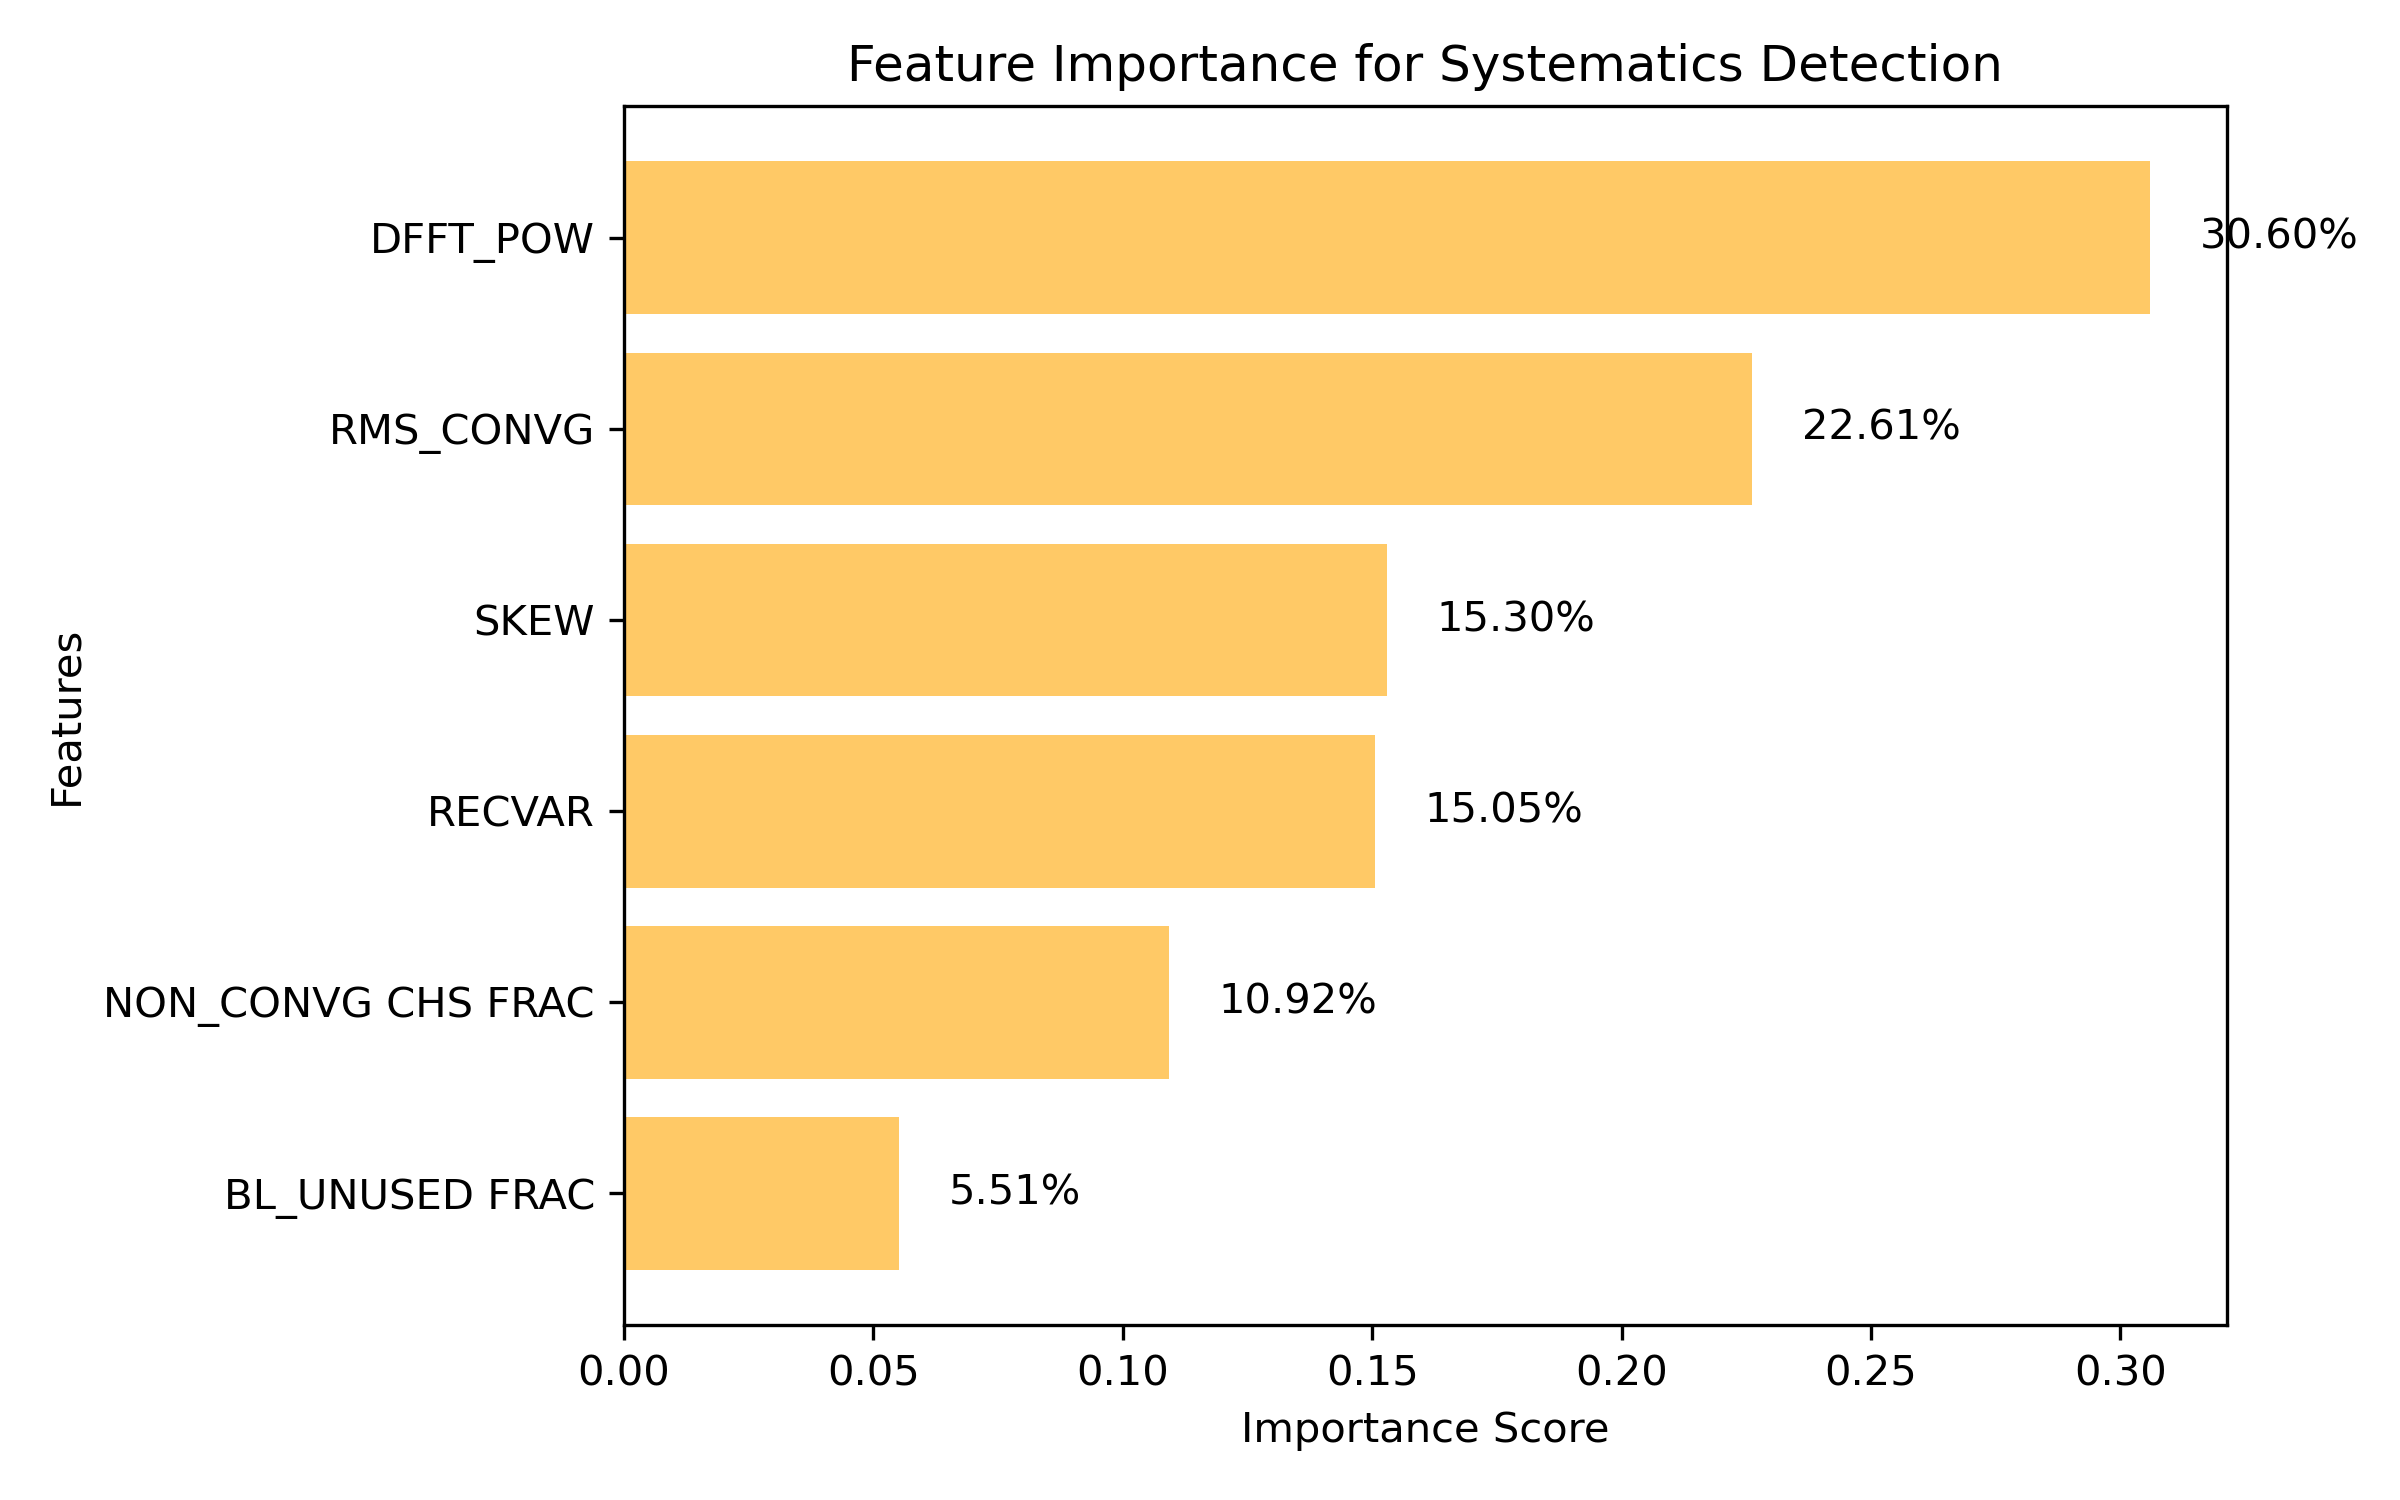
\includegraphics[width=0.8\textwidth]{features.png}
    \caption{Contribution of the different calibration parameters in reaching the outcomes.}
    \label{fig:feature_importance}
\end{figure}

\section{Scientific Implications for Epoch of Reionization Studies}
In EoR science, even small systematic contamination can significantly bias power spectrum estimation and interfere with extraction of the faint cosmological 21 cm signal. Undetected systematic errors may:
\begin{itemize}
\item Introduce false astrophysical signatures
\item Suppress weak cosmological signals
\item Bias foreground subtraction procedures
\item Propagate uncertainty into downstream scientific interpretation
\end{itemize}
Automated anomaly detection frameworks provide an essential safeguard by identifying problematic observations before inclusion in final scientific analysis. Such approaches will become increasingly important for next-generation instruments such as the Square Kilometre Array Observatory.

\section{Conclusion}
This study demonstrates the feasibility of applying machine learning techniques to detect systematic contamination in radio astronomy calibration datasets. Results show that:
\begin{itemize}
\item Calibration metrics provide meaningful information regarding observational quality.
\item Unsupervised anomaly detection alone struggles with subtle systematic failures.
\item Supervised tree-based classifiers achieve significantly improved performance.
\item Hybrid anomaly detection frameworks can identify hidden systematic contamination beyond existing labels.
\end{itemize}
Future work should focus on validating the framework using Phase III observations and extending the anomaly detection system to incorporate additional observational and instrumental metrics. Reliable identification of systematically contaminated observations represents a critical step toward improving the robustness of EoR signal detection in future radio astronomy experiments.
% \subsubsection{Extremely wide tables}

% Since PASP is now all electronic with no print version there is no reason why tables can not be as wide as authors need them to be. For wide tables, the full table will almost always be available in machine readable format with just an example in the article but how is an example created for a wide table?

% There are two ways to create examples for wide tabular data sets. The first is to to break a table into two or three components so that it flows down a page by invoking a new table type, splittabular or splitdeluxetable. Within these tables a new ``B'' column separator is introduced.  Much like the vertical bar option, ``$\vert$'', that produces a vertical table lines the new ``B'' separator indicates where to \underline{B}reak a table.  Up to two ``B''s may be included.

% Table 1 shows how to split a wide deluxetable into three parts with
% the {\tt\string\splitdeluxetable} command.  The {\tt\string\colnumbers}
% option is on to show how the automatic column numbering carries through the
% second table component.

% \begin{splitdeluxetable*}{lccccBcccccBcccc}
% \tabletypesize{\scriptsize}
% \tablewidth{0pt} 
% \tablecaption{Measurements of Emission Lines: two breaks \label{tab:deluxesplit}}
% \tablehead{
% \colhead{Model} & \colhead{Component}& \colhead{Shift} & \colhead{FWHM} &
% \multicolumn{10}{c}{Flux} \\
% \colhead{} & \colhead{} & \colhead{($\rm
% km~s^{-1}$)}& \colhead{($\rm km~s^{-1}$)} & \multicolumn{10}{c}{($\rm
% 10^{-17}~erg~s^{-1}~cm^{-2}$)} \\
% \cline{5-14}
% \colhead{} & \colhead{} &
% \colhead{} & \colhead{} & \colhead{Ly$\alpha$} & \colhead{N\,{\footnotesize
% V}} & \colhead{Si\,{\footnotesize IV}} & \colhead{C\,{\footnotesize IV}} &
% \colhead{Mg\,{\footnotesize II}} & \colhead{H$\gamma$} & \colhead{H$\beta$}
% & \colhead{H$\alpha$} & \colhead{He\,{\footnotesize I}} &
% \colhead{Pa$\gamma$}
% } 
% \colnumbers
% \startdata 
% {       }& BELs& -97.13 &    9117$\pm      38$&    1033$\pm      33$&$< 35$&$<     166$&     637$\pm      31$&    1951$\pm      26$&     991$\pm 30$&    3502$\pm      42$&   20285$\pm      80$&    2025$\pm     116$& 1289$\pm     107$\\ 
% {Model 1}& IELs& -4049.123 & 1974$\pm      22$&    2495$\pm      30$&$<     42$&$<     109$&     995$\pm 186$&      83$\pm      30$&      75$\pm      23$&     130$\pm      25$& 357$\pm      94$&     194$\pm      64$& 36$\pm      23$\\
% {       }& NELs& \nodata &     641$\pm       4$&     449$\pm 23$&$<      6$&$<       9$&       --            &     275$\pm      18$& 150$\pm      11$&     313$\pm      12$&     958$\pm      43$&     318$\pm 34$& 151$\pm       17$\\
% \hline
% {       }& BELs& -85 &    8991$\pm      41$& 988$\pm      29$&$<     24$&$<     173$&     623$\pm      28$&    1945$\pm 29$&     989$\pm      27$&    3498$\pm      37$&   20288$\pm      73$& 2047$\pm     143$& 1376$\pm     167$\\
% {Model 2}& IELs& -51000 &    2025$\pm      26$& 2494$\pm      32$&$<     37$&$<     124$&    1005$\pm     190$&      72$\pm 28$&      72$\pm      21$&     113$\pm      18$&     271$\pm      85$& 205$\pm      72$& 34$\pm      21$\\
% {       }& NELs& 52 &     637$\pm      10$&     477$\pm 17$&$<      4$&$<       8$&       --            &     278$\pm      17$& 153$\pm      10$&     317$\pm      15$&     969$\pm      40$&     325$\pm 37$&
%      147$\pm       22$\\
% \enddata
% \tablecomments{This is an example of how to split a deluxetable. You can
% split any table with this command into two or three parts.  The location of
% the split is given by the author based on the placement of the ``B''
% indicators in the column identifier preamble.  For more information please
% look at the new \aastex\ instructions.}
% \end{splitdeluxetable*}

% The second way is to create a "descriptive" table instead. This type of table only provides information about the columns rather than the data itself. Table 2 shows an example of this type of table using the same columns as in Table 1. Since these types of tables always have a machine readable component, this table uses the {\tt\string \digitalasset}\ command to highlight this fact.

% \begin{deluxetable*}{rlll}
% \digitalasset
% \tablewidth{0pt}
% \tablecaption{Descriptive version of the "Measurements of Emission Lines" table \label{tab:description}}
% \tablehead{
% \colhead{Number} & \colhead{Units} & \colhead{Label} & \colhead{Explanation}
% }
% \startdata
% 1 & --- & Model & Model identifier \\
% 2 & --- & Component & Component identifier \\
% 3 & $\rm km~s^{-1}$ & Shift & Line shift \\
% 4 & $\rm km~s^{-1}$ & FWHM & Line Full-Width at Half-Maximum \\
% 5 & $\rm 10^{-17}~erg~s^{-1}~cm^{-2}$ & Ly$\alpha$ & Ly$\alpha$ line flux \\
% 6 & $\rm 10^{-17}~erg~s^{-1}~cm^{-2}$ & N\,{\footnotesize V} & N\,{\footnotesize V} line flux \\
% 7 & $\rm 10^{-17}~erg~s^{-1}~cm^{-2}$ & Si\,{\footnotesize IV} & Si\,{\footnotesize IV} line flux \\
% 8 & $\rm 10^{-17}~erg~s^{-1}~cm^{-2}$ & C\,{\footnotesize IV} & C\,{\footnotesize IV} line flux \\
% 9 & $\rm 10^{-17}~erg~s^{-1}~cm^{-2}$ & Mg\,{\footnotesize II} & Mg\,{\footnotesize II} line flux \\
% 10 & $\rm 10^{-17}~erg~s^{-1}~cm^{-2}$ & H$\gamma$ & H$\gamma$ line flux \\
% 11 & $\rm 10^{-17}~erg~s^{-1}~cm^{-2}$ & H$\beta$ & H$\beta$ line flux \\
% 12 & $\rm 10^{-17}~erg~s^{-1}~cm^{-2}$ & H$\alpha$ & H$\alpha$ line flux \\
% 13 & $\rm 10^{-17}~erg~s^{-1}~cm^{-2}$ & He\,{\footnotesize I} & He\,{\footnotesize I} line flux \\
% 14 & $\rm 10^{-17}~erg~s^{-1}~cm^{-2}$ & Pa$\gamma$ & Pa$\gamma$ line flux \\
% \enddata
% \tablecomments{Table 2 is published in its entirety in the electronic 
% edition of the {\it Astrophysical Journal}.  A portion is shown here 
% for guidance regarding its form and content. The {\tt\string \digitalasset}\ command highlights the Table title to visually indicate to the reader that there is data associated with this table.}
% \end{deluxetable*}

% \subsection{Figures\label{subsec:figures}}

% Authors can include a wide number of different graphics with their articles.
% These range from general figures all authors are familiar with
% to new enhanced graphics that can only be fully experienced in HTML.  The
% later include figure sets, animations and interactive figures.  All
% enhanced graphics require a static two dimensional representation in the
% manuscript to serve as the example for the reader. All figures should
% include detailed and descriptive captions.  These captions are absolutely
% critical for readers for whom the enhanced figure is inaccessible either
% due to a disability or offline access.  This portion of the article
% provides examples for setting up all these types in with the latest version
% of \aastex.

% \subsection{General figures\label{subsec:general}}

% %% The "ht!" tells LaTeX to put the figure "here" first, at the "top" next
% %% and to override the normal way of calculating a float position.
% %% The asterisk after "figure" tells the compiler to span multiple columns
% %% if a two column style is selected.
% \begin{figure}[ht!]
% \plotone{KwitterHenryPASPReviewPN2022-Figure3.jpg}
% \caption{Hertzsprung–Russell diagram of a complete evolutionary track for a 2 M$_\odot$ solar-metallicity star from the main sequence to the white dwarf phase.  From \cite{Kwitter2022PASP}.
% \label{fig:general}}
% \end{figure}

% \aastex\ has a {\tt\string\plotone} command to display a figure consisting
% of one figure file.  Figure \ref{fig:general} is an example. For a general figure
% consisting of two figure files the {\tt\string\plottwo} command can be
% used to position the two image files side by side.

% Both {\tt\string\plotone} and {\tt\string\plottwo} take a
% {\tt\string\caption} and an optional {\tt\string\figurenum} command to
% specify the figure number\footnote{It is better to not use
% {\tt\string\figurenum} and let \latex\ auto-increment all the figures. If you
% do use this command you need to mark all of them accordingly.}.  Each is
% based on the {\tt\string graphicx} package command,
% {\tt\string\includegraphics}.  Authors are welcome to use
% {\tt\string\includegraphics} along with its optional arguments that control
% the height, width, scale, and position angle of a file within the figure.
% More information on the full usage of {\tt\string\includegraphics} can be
% found at \break
% \url{https://en.wikibooks.org/wiki/LaTeX/Importing\_Graphics\#Including\_graphics}.

% \subsection{Enhanced graphics}

% Enhanced graphics have an example figure to serve as an example for the
% reader and the full graphical item available in the published HTML article.
% This includes Figure sets, animations, and interactive figures. The 
% Astronomy Image Explorer (\url{http://www.astroexplorer.org/}) provides 
% access to all the figures published in the AAS Journals since they offered
% an electronic version which was in the mid 1990s. You can filter image
% searches by specific terms, year, journal, or type. The type filter is 
% particularly useful for finding all published enhanced graphics. As of
% August 2024 there are over 5600 videos, 2200 figure sets, and 200 interactive
% figures. The next sections describe how to include these types of graphics
% in your own manuscripts.

% \section{Revision tracking and color highlighting} \label{sec:highlight}

% The {\tt\string\added\{<text>\}} command should be used to highlight new text in bold for revised manuscripts. To activate this command, the {\tt\string trackchanges} option must be used in the {\tt\string\documentclass} call.  When compiled this will produce the marked text in bold font. Take out the {\tt\string trackchanges} option if you want the bold to disappear.

% \added{This text was specifically added to feature this reborn functionality. Notice how the bold goes away when you remove the 'trackfeatures' option.}

% \section{Software and third party data repository citations} \label{sec:cite}

% PASP would like to encourage authors to change software and
% third party data repository references from the current standard of a
% footnote to a first class citation in the bibliography.  As a bibliographic
% citation these important references will be more easily captured and credit
% will be given to the appropriate people.

% The first step to making this happen is to have the data or software in
% a long term repository that has made these items available via a persistent
% identifier like a Digital Object Identifier (DOI).  A list of repositories
% that satisfy this criteria plus each one's pros and cons are given at \break
% \url{https://github.com/AASJournals/Tutorials/tree/master/Repositories}.

% In the bibliography the format for data or code follows this format: \\

% \noindent author year, title, version, publisher, prefix:identifier\\

% \citet{2015ApJ...805...23C} provides a example of how the citation in the
% article references the external code at
% \doi{10.5281/zenodo.15991}.  Unfortunately, bibtex does
% not have specific bibtex entries for these types of references so the
% ``@misc'' type should be used.  The Repository tutorial explains how to
% code the ``@misc'' type correctly.  The most recent .bst file, aasjournalv7.bst, will output bibtex ``@misc'' type properly.

% Authors can also use the website \url{https://www.doi2bib.org/} to create a BIBTeX entry for any DOI. Please check the output from this site carefully as its output is only as good as the DOI metadata. Some DOI creators do not provide enough metadata to construct an adequate citation.

% %% Please use the acknowledgment and contribution environments. This will 
% %% be anonomyized when the "anonymous" style option is used. 
% \begin{acknowledgments}
% We thank all the people that have made this AASTeX what it is today.  This
% includes but not limited to Bob Hanisch, Chris Biemesderfer, Lee Brotzman,
% Pierre Landau, Arthur Ogawa, Maxim Markevitch, Alexey Vikhlinin and Amy
% Hendrickson. Also special thanks to David Hogg and Daniel Foreman-Mackey
% for the new {\tt\string modern} style design. Considerable help was provided via bug
% reports and hacks from numerous people including Patricio Cubillos, Alex
% Drlica-Wagner, Sean Lake, Michele Bannister, Peter Williams, Jonathan
% Gagne, Arthur Adams, Nicholas Wogan, Aaron Pearlman, Jeff Mangum, Mark Durre, Joel Ong, and Stephen Thorp.
% \end{acknowledgments}

% \begin{contribution}
% %%This section gives authors the space to recognize author contributions. The text inside this environment is NOT counted towards the total word quanta. At a minimum, manuscripts are expected to include this text:

% All editors contribute equally to the operation of PASP.

% %% But authors are expected to provide more specific details, e.g. 
% %%
% %%SC was responsible for writing and submitting the manuscript.
% %%WWM came up with the initial research concept and edited the manuscript.
% %%OTS obtained the funding and edited the manuscript.
% %%EBF provided the formal analysis and validation. He also edited the manuscript.
% %%GEH Supervised the undergraduates, wrote the software and administers the project github and Zenodo repositories.
% %%
% %% Authors can use the Contributor Role Taxonomy (CRediT) at
% %% https://credit.niso.org
% %% for ideas on how write a good statement tailored to their needs.

% \end{contribution}

% %% To help institutions obtain information on the effectiveness of their 
% %% telescopes the AAS Journals has created a group of keywords for telescope 
% %% facilities.
% %
% %% Following the acknowledgments section, use the following syntax and the
% %% \facility{} or \facilities{} macros to list the keywords of facilities used 
% %% in the research for the paper.  Each keyword is check against the master 
% %% list during copy editing.  Individual instruments can be provided in 
% %% parentheses, after the keyword, but they are not verified.
% \facilities{HST(STIS), Swift(XRT and UVOT), AAVSO, CTIO:1.3m, CTIO:1.5m, CXO}

% %% Similar to \facility{}, there is the optional \software command to allow 
% %% authors a place to specify which programs were used during the creation of 
% %% the manuscript. Authors should list each code and include either a
% %% citation or url to the code inside ()s when available.
% \software{astropy \citep{2013A&A...558A..33A,2018AJ....156..123A,2022ApJ...935..167A},  
%           Cloudy \citep{2013RMxAA..49..137F}, 
%           Source Extractor \citep{1996A&AS..117..393B}
%           }

% %% Appendix material should be preceded with a single \appendix command.
% %% There should be a \section command for each appendix. Mark appendix
% %% subsections with the same markup you use in the main body of the paper.
% %%
% %% Each Appendix (indicated with \section) will be lettered A, B, C, etc.
% %% The equation counter will reset when it encounters the \appendix
% %% command and will number appendix equations (A1), (A2), etc. The
% %% Figure and Table counter will not reset.

% \appendix

% \section{Appendix information}

% Appendices can be broken into separate sections just like in the main text.
% The only difference is that each appendix section is indexed by a letter
% (A, B, C, etc.) instead of a number.  Likewise numbered equations have
% the section letter appended.  Here is an equation as an example.
% \begin{equation}
% I = \frac{1}{1 + d_{1}^{P (1 + d_{2} )}}
% \end{equation}
% Appendix tables and figures should not be numbered like equations. Instead
% they should continue the sequence from the main article body.

% \section{Author publication charges} \label{sec:pubcharge}

% PASP is a hybrid open access journal. Authors have the option to pay article publication charge (APC) to publish their article on an open access basis under a Creative Commons Attribution (CC BY) license. Additionally, PASP is supported in part by page charges.  The current cost
% for publication charges is available at 
% \url{https://iopscience.iop.org/journal/1538-3873/page/publication-charges}. 

% \section{Rotating tables} \label{sec:rotate}

% To place a single page table in a landscape mode start the table portion with {\tt\string\begin\{rotatetable\}} and end with {\tt\string\end\{rotatetable\}}.

% Tables that exceed a print page take a slightly different environment since both rotation and long table printing are required. In these cases start with {\tt\string\begin\{longrotatetable\}} and end with {\tt\string\end\{longrotatetable\}}. The {\tt\string\movetabledown} command can be used to help center extremely wide, landscape tables. The command {\tt\string\movetabledown=1in} will move any rotated table down 1 inch. 

% A handy "cheat sheet" that provides the necessary \latex\ to produce 17
% different types of tables is available at \url{http://journals.aas.org/authors/aastex/aasguide.html#table_cheat_sheet}.

% \section{Using Chinese, Japanese, and Korean characters}

% Authors have the option to include names in Chinese, Japanese, or Korean (CJK)
% characters in addition to the English name. The names will be displayed
% in parentheses after the English name. The way to do this in AASTeX is to
% use the CJK package available at \url{https://ctan.org/pkg/cjk?lang=en}.
% Further details on how to implement this and solutions for common problems,
% please go to \url{https://journals.aas.org/nonroman/}.

% %% For this sample we use BibTeX plus aasjournalv7.bst to generate the
% %% the bibliography. The sample7.bib file was populated from ADS. To
% %% get the citations to show in the compiled file do the following:
% %%
% %% pdflatex sample7.tex
% %% bibtext sample7
% %% pdflatex sample7.tex
% %% pdflatex sample7.tex

\bibliography{PASPsample701}{}
\bibliographystyle{aasjournalv7}

%% This command is needed to show the entire author+affiliation list when
%% the collaboration and author truncation commands are used.  It has to
%% go at the end of the manuscript.
%\allauthors

%% Include this line if you are using the \added, \replaced, \deleted
%% commands to see a summary list of all changes at the end of the article.
%\listofchanges

\end{document}

% End of file `PASPsample701.tex'.
